\documentclass{beamer}
\usepackage[utf8]{inputenc}

\usepackage[citestyle=authoryear,bibstyle=authoryear,natbib]{biblatex}
\addbibresource{Sources.bib}

\usepackage{array}
\usepackage{graphicx}
\usepackage{xcolor}
\usepackage{pgfplots}
\pgfplotsset{compat=1.13}
\usepackage{tikz}
\usetikzlibrary{arrows,arrows.meta,patterns,matrix,shapes,calc,positioning}
\usepackage{amsmath,amssymb,amsthm}

\usepackage{import}
\usepackage{catchfile}
\newcommand\loaddata[1]{\CatchFileDef\loadeddata{#1}{\endlinechar=-1}}

\newlength{\rs}

\definecolor{Rred}   {RGB}{191, 63, 63}%BF1F7F
\definecolor{Rgreen} {RGB}{ 63,191, 63}%1FBF1F
\definecolor{Rblue}  {RGB}{ 63, 63,255}%1F1FBF

\definecolor{Rpink}  {RGB}{255, 31,127}%FF1F7F
\definecolor{Rpurple}{RGB}{127, 31,255}%7F1FFF
\definecolor{Rorange}{RGB}{255,127, 31}%FF7F1F
\definecolor{Rlime}  {RGB}{127,255, 31}%7FFF1F
\definecolor{Rocean} {RGB}{ 31,127,255}%1F7FFF
\definecolor{Raqua}  {RGB}{ 31,255,127}%1FFF7F

\title{Neural Networks with Python and TensorFlow}
\author{Alexander J. Johnson}
\institute{Manchester Metropolitan University}
\date{2020}


\begin{document}

\frame{\titlepage}

\begin{frame}
    \frametitle{Aims and Objectives}

    \begin{itemize}
        \item Provide an introduction to a variety of neural network
            architectures.
        \item Implement the architectures in python using TensorFlow.
        \item Use neural networks to solve simple problems.
    \end{itemize}
\end{frame}

\begin{frame}
    \frametitle{Basis}

    Biological Neuron:
    \begin{center}
        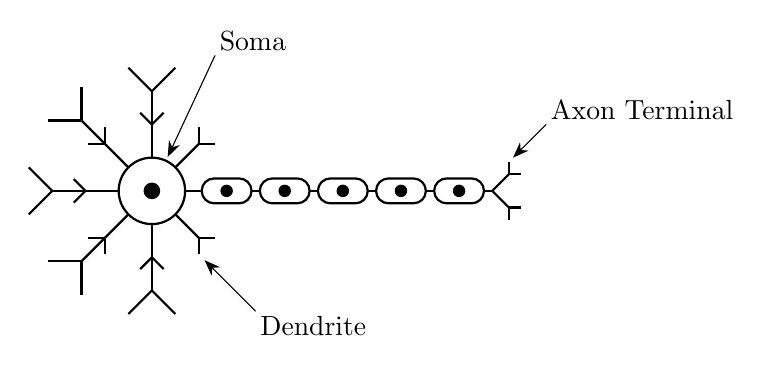
\begin{tikzpicture}%[x=1pt,y=1pt]
    [   > = {Stealth[scale=1.2]}
    ]
    \setlength{\rs}{1.5pt}
    % Nucleus
    \fill (0\rs,0\rs) circle (2\rs);
    % Soma
    \draw[thick] (0\rs,0\rs) circle (8\rs);
    % Dendrite
    \draw[thick] ( 45:8\rs) -- ( 45:16\rs);
        \draw[thick] ( 45:16\rs) -- ++(  0:4\rs);
        \draw[thick] ( 45:16\rs) -- ++( 90:4\rs);
    \draw[thick] ( 90:8\rs) -- ( 90:24\rs);
        \draw[thick] ( 90:16\rs) -- ++( 45:4\rs);
        \draw[thick] ( 90:16\rs) -- ++(135:4\rs);
        \draw[thick] ( 90:24\rs) -- ++( 45:8\rs);
        \draw[thick] ( 90:24\rs) -- ++(135:8\rs);
    \draw[thick] (135:8\rs) -- (135:24\rs);
        \draw[thick] (135:16\rs) -- ++( 90:4\rs);
        \draw[thick] (135:16\rs) -- ++(180:4\rs);
        \draw[thick] (135:24\rs) -- ++( 90:8\rs);
        \draw[thick] (135:24\rs) -- ++(180:8\rs);
    \draw[thick] (180:8\rs) -- (180:24\rs);
        \draw[thick] (180:16\rs) -- ++(135:4\rs);
        \draw[thick] (180:16\rs) -- ++(225:4\rs);
        \draw[thick] (180:24\rs) -- ++(135:8\rs);
        \draw[thick] (180:24\rs) -- ++(225:8\rs);
    \draw[thick] (225:8\rs) -- (225:24\rs);
        \draw[thick] (225:16\rs) -- ++(180:4\rs);
        \draw[thick] (225:16\rs) -- ++(270:4\rs);
        \draw[thick] (225:24\rs) -- ++(180:8\rs);
        \draw[thick] (225:24\rs) -- ++(270:8\rs);
    \draw[thick] (270:8\rs) -- (270:24\rs);
        \draw[thick] (270:16\rs) -- ++(225:4\rs);
        \draw[thick] (270:16\rs) -- ++(315:4\rs);
        \draw[thick] (270:24\rs) -- ++(225:8\rs);
        \draw[thick] (270:24\rs) -- ++(315:8\rs);
    \draw[thick] (315:8\rs) -- (315:16\rs);
        \draw[thick] (315:16\rs) -- ++(270:4\rs);
        \draw[thick] (315:16\rs) -- ++(360:4\rs);
    % Axon
    \draw[thick] (8\rs,0\rs) -- (12\rs,0\rs);
    \draw[thick,rounded corners=3\rs] (12\rs,-3\rs) rectangle (24\rs,3\rs);
        \fill (18\rs,0\rs) circle (1.5\rs);
    \draw[thick] (24\rs,0\rs) -- (26\rs,0\rs);
    \draw[thick,rounded corners=3\rs] (26\rs,-3\rs) rectangle (38\rs,3\rs);
        \fill (32\rs,0\rs) circle (1.5\rs);
    \draw[thick] (38\rs,0\rs) -- (40\rs,0\rs);
    \draw[thick,rounded corners=3\rs] (40\rs,-3\rs) rectangle (52\rs,3\rs);
        \fill (46\rs,0\rs) circle (1.5\rs);
    \draw[thick] (52\rs,0\rs) -- (54\rs,0\rs);
    \draw[thick,rounded corners=3\rs] (54\rs,-3\rs) rectangle (66\rs,3\rs);
        \fill (60\rs,0\rs) circle (1.5\rs);
    \draw[thick] (66\rs,0\rs) -- (68\rs,0\rs);
    \draw[thick,rounded corners=3\rs] (68\rs,-3\rs) rectangle (80\rs,3\rs);
        \fill (74\rs,0\rs) circle (1.5\rs);
    % Axon terminal
    \draw[thick] (80\rs,0\rs) -- (82\rs,0\rs);
        \draw[thick] (82\rs,0\rs) -- (86\rs,4\rs);
            \draw[thick] (86\rs,4\rs) -- (86\rs,7\rs);
            \draw[thick] (86\rs,4\rs) -- (89\rs,4\rs);
        \draw[thick] (82\rs,0\rs) -- (86\rs,-4\rs);
            \draw[thick] (86\rs,-4\rs) -- (86\rs,-7\rs);
            \draw[thick] (86\rs,-4\rs) -- (89\rs,-4\rs);
    % Labels
    % Soma
    \draw[<-] (65:9\rs) -- (65:36\rs);
    \node[anchor=south west,inner sep=1\rs] at (65:36\rs) {Soma};
    % Dendrite
    %\draw[latex'-] (225:25\rs) -- (225:36\rs);
    \draw[<-] (12.7\rs,-16.7\rs) -- (25\rs,-29\rs);
    \node[anchor=north west,inner sep=1\rs] at (25\rs,-29\rs) {Dendrite};
    % Axon Terminal
    \draw[<-] (87\rs,8\rs) -- (95\rs,16\rs);
    \node[anchor=south west,inner sep=1\rs] at (95\rs,16\rs) {Axon Terminal};
\end{tikzpicture}

    \end{center}
    Receives signals via dendrites and soma,
    applies threshold,
    outputs via axon terminal.
\end{frame}

\begin{frame}
    \frametitle{Perceptron}

    \cite{Rosenblatt:1958:Perceptron}:
    \begin{align*}
        A_i = \begin{cases}
            1, & \sum_j w_{i,j}x_j > \theta\\
            0, & \text{otherwise}
        \end{cases}
    \end{align*}

    Boolean output.

    Weights adjusted according to activation and response correctness.
\end{frame}

\begin{frame}
    \frametitle{Modern Neural Network}

    Most common activation equation outlined by \cite{McClelland:1986:Parallel}:
    \begin{align*}
        y_i = \phi \left(b + \sum_j w_{i,j}x_j\right).
    \end{align*}

    Weights adjusted via backpropagation / chain rule:
    \begin{align*}
        w_i' = w_i + \eta\frac{\partial f}{\partial w_i}.
    \end{align*}

    Supported out-of-the-box by TensorFlow.
\end{frame}

\begin{frame}
    \frametitle{Convolutional}

    Original concept by \cite{Fukushima:1980:Neocognitron}.

    Features of convolutional layers:
    \begin{itemize}
        \item Neurons only connect to regions of previous layers.
        \item Share same weight scheme.
        \item Implicitly encodes position.
        \item Shift invariant, useful in image processing.
    \end{itemize}

    Supported out-of-the-box by TensorFlow.
\end{frame}

\begin{frame}
    \frametitle{Convolutional}

    \begin{center}
        \begin{tikzpicture}
    \loaddata{../Code/CharacterRecognition/PosterFigrFlat.txt}
    \foreach\posx/\posy/\pred/\cert/\actu in \loadeddata
    {   \pgfmathtruncatemacro{\indx}{5*\posy+\posx}
        \node[draw] (N\indx) at (3*\posx,0)
        {\includegraphics[width=20mm]{CRResults/img\indx}};
        \node (P\indx) at (N\indx.north) [anchor=south]
        {\scriptsize Predicted: \pred};
        \node (A\indx) at (P\indx.north) [anchor=south,outer sep=0,inner sep=0]
        {\scriptsize Was: \actu};
        \node (S\indx) at (N\indx.south) [anchor=north]
        {\scriptsize \ifnum \actu=\pred
                Correct
            \else
                \underline{\textbf{Incorrect}}
            \fi};
        \node (C\indx) at (S\indx.south) [anchor=north,outer sep=0,inner sep=0]
        {\scriptsize Certainty: \cert};
    }
\end{tikzpicture}

    \end{center}
    Character recognition for the MNIST dataset using a convolutional neural
    network.
\end{frame}

\begin{frame}
    \frametitle{Recurrent}

    Features of recurrent layers:
    \begin{itemize}
        \item Has an internal state.
        \item Useful for temporal tasks.
        \item Suitable for both short and long time scales.
    \end{itemize}

    Supported out-of-the-box by TensorFlow.
\end{frame}

\begin{frame}
    \frametitle{Reinforcement Learning}

    Example: Chain problem from \cite{Strens:2000:ABF}.
    \begin{center}
        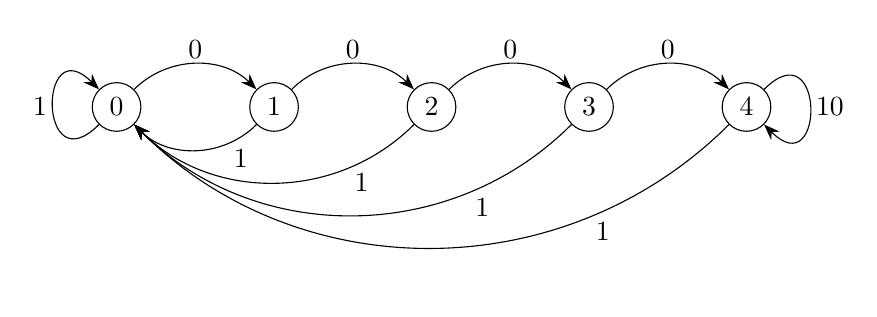
\begin{tikzpicture}
    [   state/.style=
        {   draw
        ,   circle
        }
    ,   baseline=0pt
    ,   >={Stealth[scale=1.2]}
    ]
    \foreach\n in {0,...,4}
    {   \node[state] (N\n) at (2cm*\n, 0mm) {$\n$};
    }
    \foreach\np in {1,...,4}
    {   \pgfmathtruncatemacro{\nm}{\np-1}
        \draw[->]
        (N\np)
            to [out=225,in=315]
            node [near start, anchor = north west, inner sep = 2pt] {1}
        (N0);
        \draw[->]
        (N\nm)
            to [out=45,in=135]
            node [anchor = south, inner sep = 2pt] {0}
        (N\np);
    }
    \draw[->]
    (N0)
        .. controls ++(-1cm,-1cm) and ++(-1cm,1cm) ..
        node [anchor = east, inner sep = 2pt] {1}
    (N0);
    \draw[->]
    (N4)
        .. controls ++(1cm,1cm) and ++(1cm,-1cm) ..
        node [anchor = west, inner sep = 2pt] {10}
    (N4);
\end{tikzpicture}

    \end{center}
\end{frame}

\begin{frame}
    \frametitle{Reinforcement Learning}

    Q-Learning \citep{Watkins:1989:Learning}:
    \begin{align*}
        Q(s,a) \leftarrow Q(s,a) + \alpha(r + \gamma\max_{a'} Q(s',a') - Q(s,a))
    \end{align*}
    Deep Q-Learning replaces table with network.

    Improvements:
    \begin{itemize}
        \item Prioritised Experience Replay.
        \item Fixed Q-Targets.
        \item Double Deep Q-Networks.
        \item Dueling Deep Q-Network.
    \end{itemize}
    Implementing Dueling Deep Q-Networks requires some additional work, but is
    relatively simple.
\end{frame}

\begin{frame}
    \frametitle{Reinforcement Learning}

    Policy Gradient \citep{Sutton:2000:Policy}:
    \begin{align*}
        \frac{\partial\rho}{\partial\theta} = \sum_s d^\pi(s)
        \sum_a \frac{\partial\pi(s,a)}{\partial\theta}Q^\pi(s,a)
    \end{align*}
    Stochastic policy instead of deterministic.

    Could not implement in TensorFlow during project due to limited informal
    resources about lower-level functions.

    Can be combined with Deep Q-Learning to create Actor-Critic methods, which
    are currently the start-of-the-art method for reinforcement learning.
\end{frame}

\begin{frame}
    \frametitle{Conclusions}

    \begin{itemize}
        \item Neural networks can be applied to a large variety of problems.
        \item TensorFlow provides an easy-to-use framework for defining and
            training models.
        \item Although well documented, TensorFlow's lower-level features and
            functions lack sufficient informal resources.
    \end{itemize}

    Project source code: \texttt{https://github.com/RanfordS/2020-Masters-Project}
\end{frame}

\begin{frame}
    \frametitle{Bibliography}
    \renewcommand*{\bibfont}{\normalfont\scriptsize}
    \printbibliography
    \begin{tikzpicture}
        [   remember picture
        ,   overlay
        ]
        \fill[white]
            ($(current page.north west) + (0pt,-1cm)$)
            rectangle
            ($(current page.south west) + (1cm,0pt)$);
    \end{tikzpicture}
\end{frame}

\end{document}
